\documentclass[11pt]{article}
\usepackage[utf8]{inputenc}
\usepackage{amsmath, amssymb}
\usepackage{graphicx}
\usepackage{hyperref}
\usepackage{geometry}
\usepackage[backend=biber]{biblatex}
\addbibresource{../references.bib}
\geometry{margin=1in}

\title{Expanding Entropy and the Birth of Spacetime}
\author{Juha Meskanen}
\date{\today}

\begin{document}
\maketitle

\begin{abstract}
    We explore the hypothesis that the growth of entropy in a computable execution trace corresponds to the expansion of spacetime, offering a natural explanation for both the low-entropy initial state of the universe and its inflationary growth. Using simple simulations based on bitstring evolution and particle definitions derived from minimal structures, we demonstrate that entropy increase drives an emergent geometric expansion. Furthermore, we observe that the statistical distribution of emergent structure probabilities follows a lognormal pattern. We also derive that the geometry of the singularity is smooth—contrary to the predictions of General Relativity.
\end{abstract}

\section{Introduction}

In previous work, we proposed an information-theoretic framework to describe the collapse of spacetime geometry through entropy reduction, formalized in the \textbf{Entropy-Singularity Lemma}: \textit{vanishing entropy implies geometric singularity} \cite{meskanen2020}.

In this paper, we reverse that process, postulating that an \textbf{increase in entropy} corresponds to the expansion of spacetime, effectively mapping the rise in informational complexity to cosmological inflation.

\section{Entropy as a Driver of Expansion}

We define an execution trace $S_t$, $t = 0 \ldots n$, where each $S_t$ is a binary string of fixed length $L$. Beginning from a state of zero entropy (an all-zero string), we evolve $S_t$ via random bit-flip mutations that incrementally increase its entropy.

Each $S_t$ is geometrically interpreted through a decoding scheme $D: \{0,1\}^L \to \mathbb{R}^d$. In this study, we define a hierarchy of elementary structures as follows:

\begin{enumerate}
    \item \textbf{Spacetime fabric:} Defined as 3D points directly encoded from the bitstring.
    \item \textbf{Elementary particles:} Defined as pairs of 3D points $(p_1, p_2)$ where the spatial separation between the points is below a threshold, suggesting interaction.
    \item \textbf{Atoms:} Defined as triplets of points $(p_1, p_2, p_3)$ such that:
          \[
              0 < \text{distance}(p_1, p_2) < \text{threshold}, \quad
              0 < \text{distance}(p_2, p_3) < \text{threshold}, \quad
              0 < \text{distance}(p_3, p_1) < \text{threshold},
          \]
          with distances approximately equal, implying a near-equilateral configuration.
    \item \textbf{Molecules:} Formed when two atoms are sufficiently close. The center of an atom is the geometric mean of its points:
          \[
              \text{center(atom)} = \left( \frac{x_1 + x_2 + x_3}{3}, \frac{y_1 + y_2 + y_3}{3}, \frac{z_1 + z_2 + z_3}{3} \right).
          \]
          A molecule forms if the distance between two atom centers is below a threshold:
          \[
              \text{distance}(\text{center}(atom_1), \text{center}(atom_2)) < \text{threshold}.
          \]
\end{enumerate}

We extract these structures from substrings of $S_t$ and count the number of distinct particles at each timestep. As entropy increases through random bit flips, we observe:

\begin{enumerate}
    \item Initially, when entropy is near zero, no valid structures are decoded.
    \item As entropy increases, the number of identifiable structures grows rapidly.
    \item This growth slows with higher entropy, mirroring inflation followed by gradual expansion.
\end{enumerate}

\begin{figure}[h!]
    \centering
    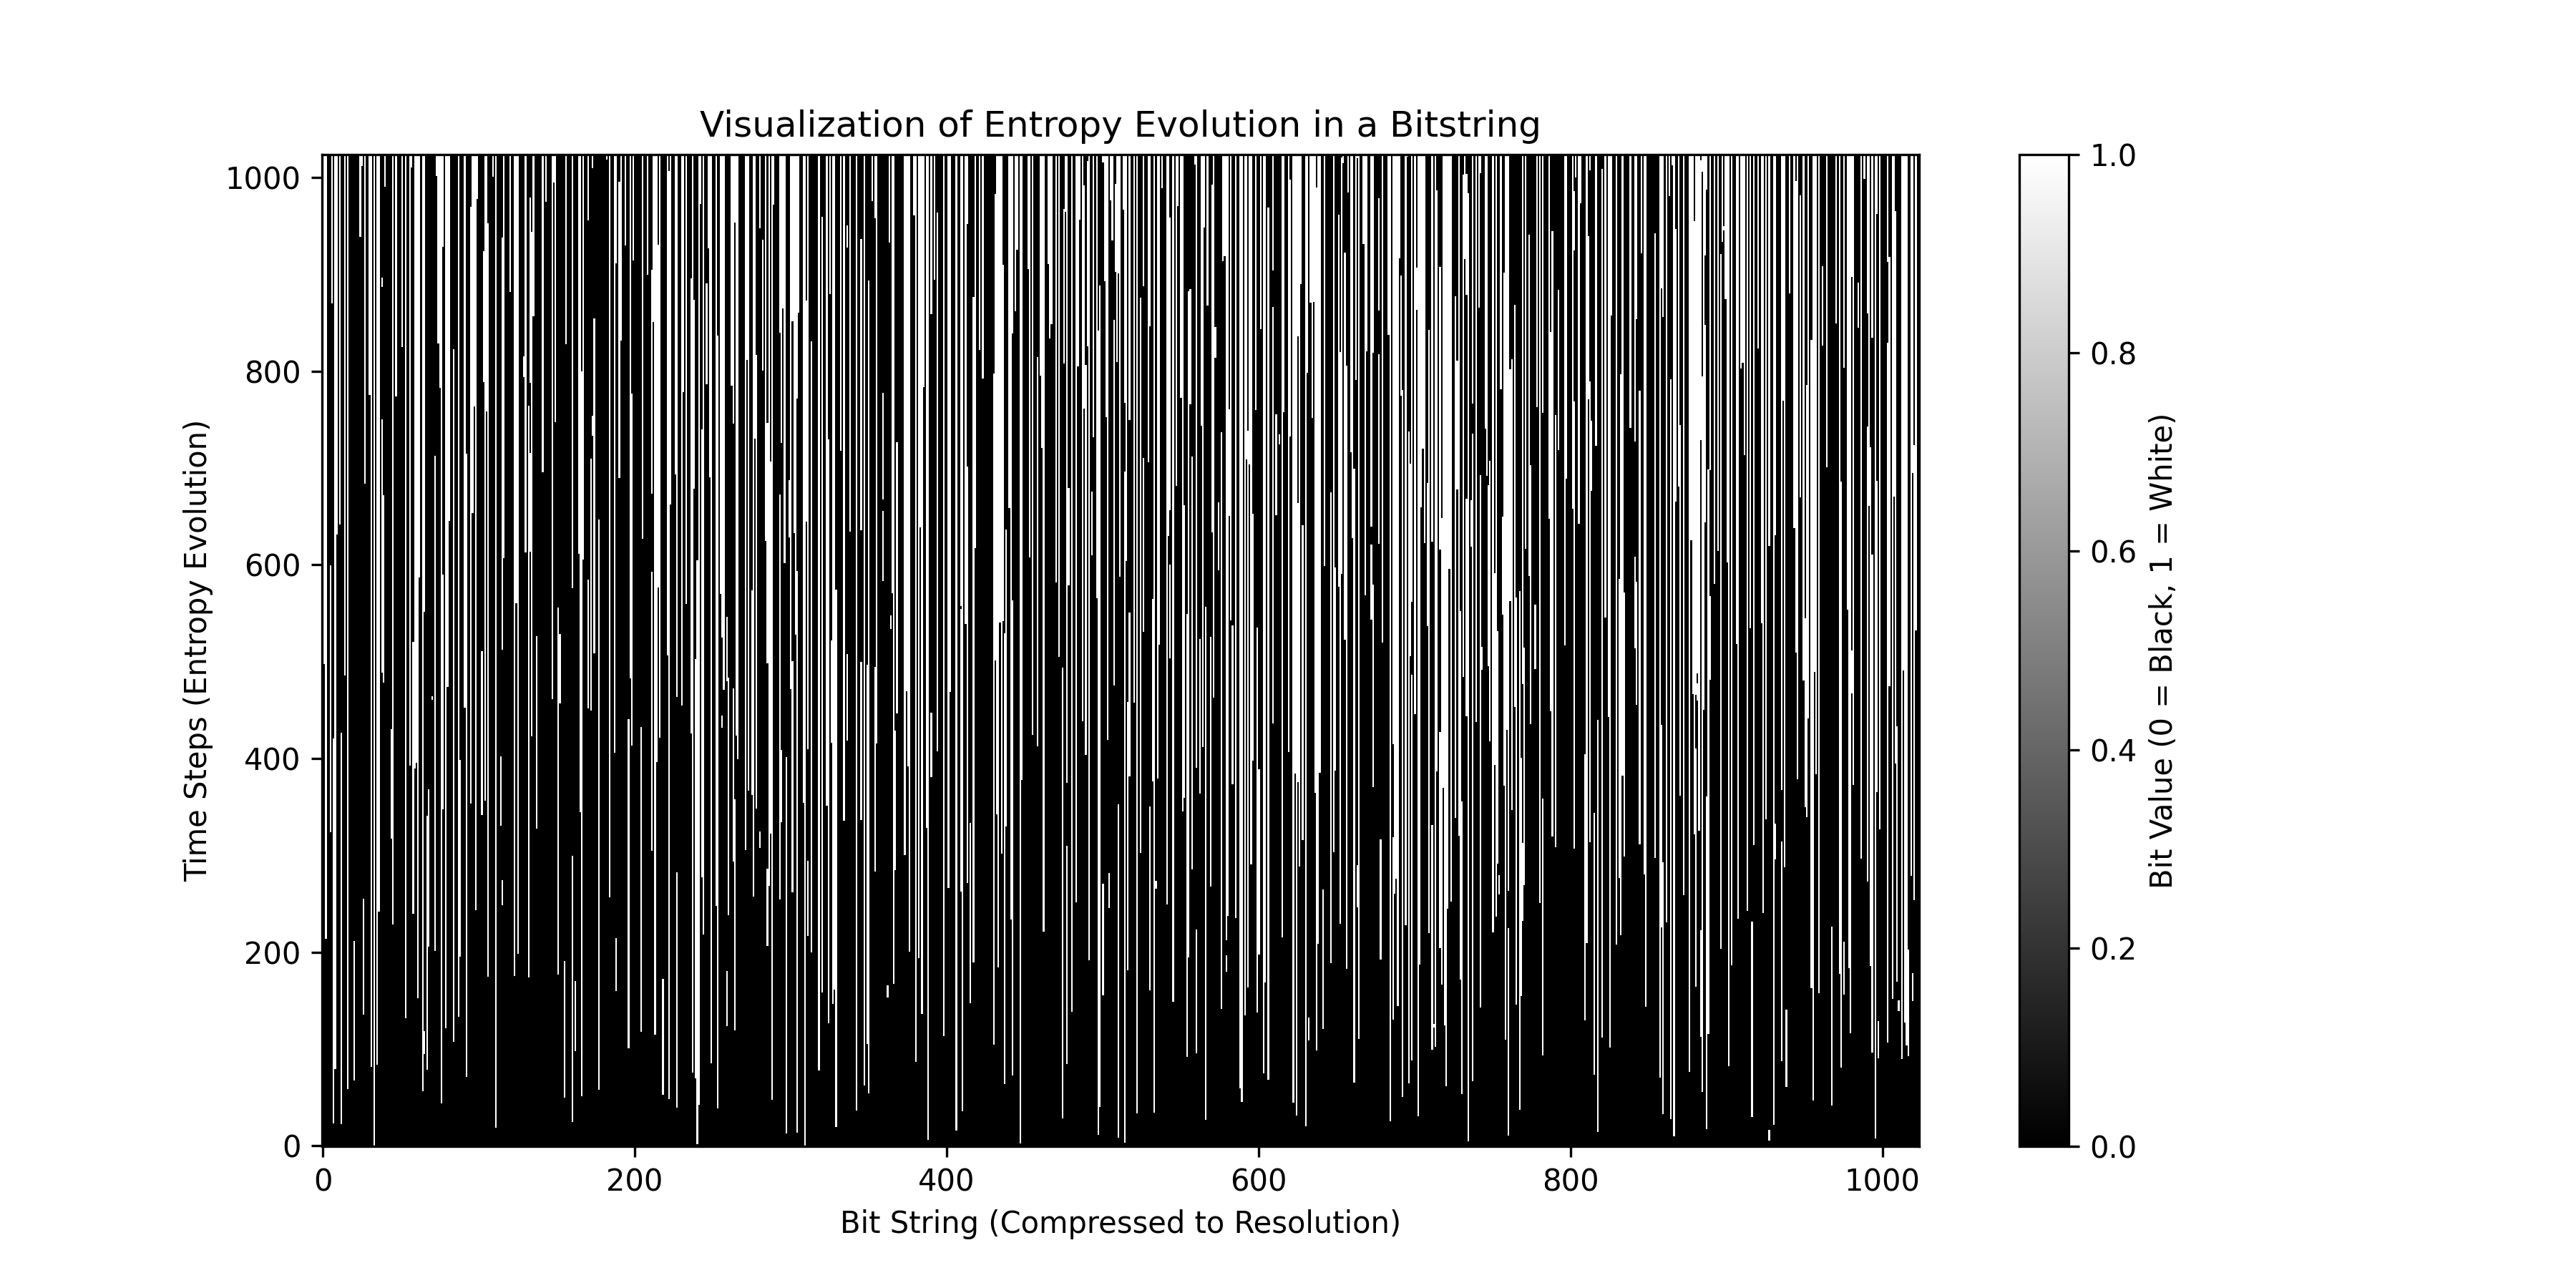
\includegraphics[width=0.8\textwidth]{figures/entropy_evolution_image.png}
    \caption{Evolution of Shannon entropy due to bit flips.}
    \label{fig:entropy-evolution}
\end{figure}

\begin{figure}[h!]
    \centering
    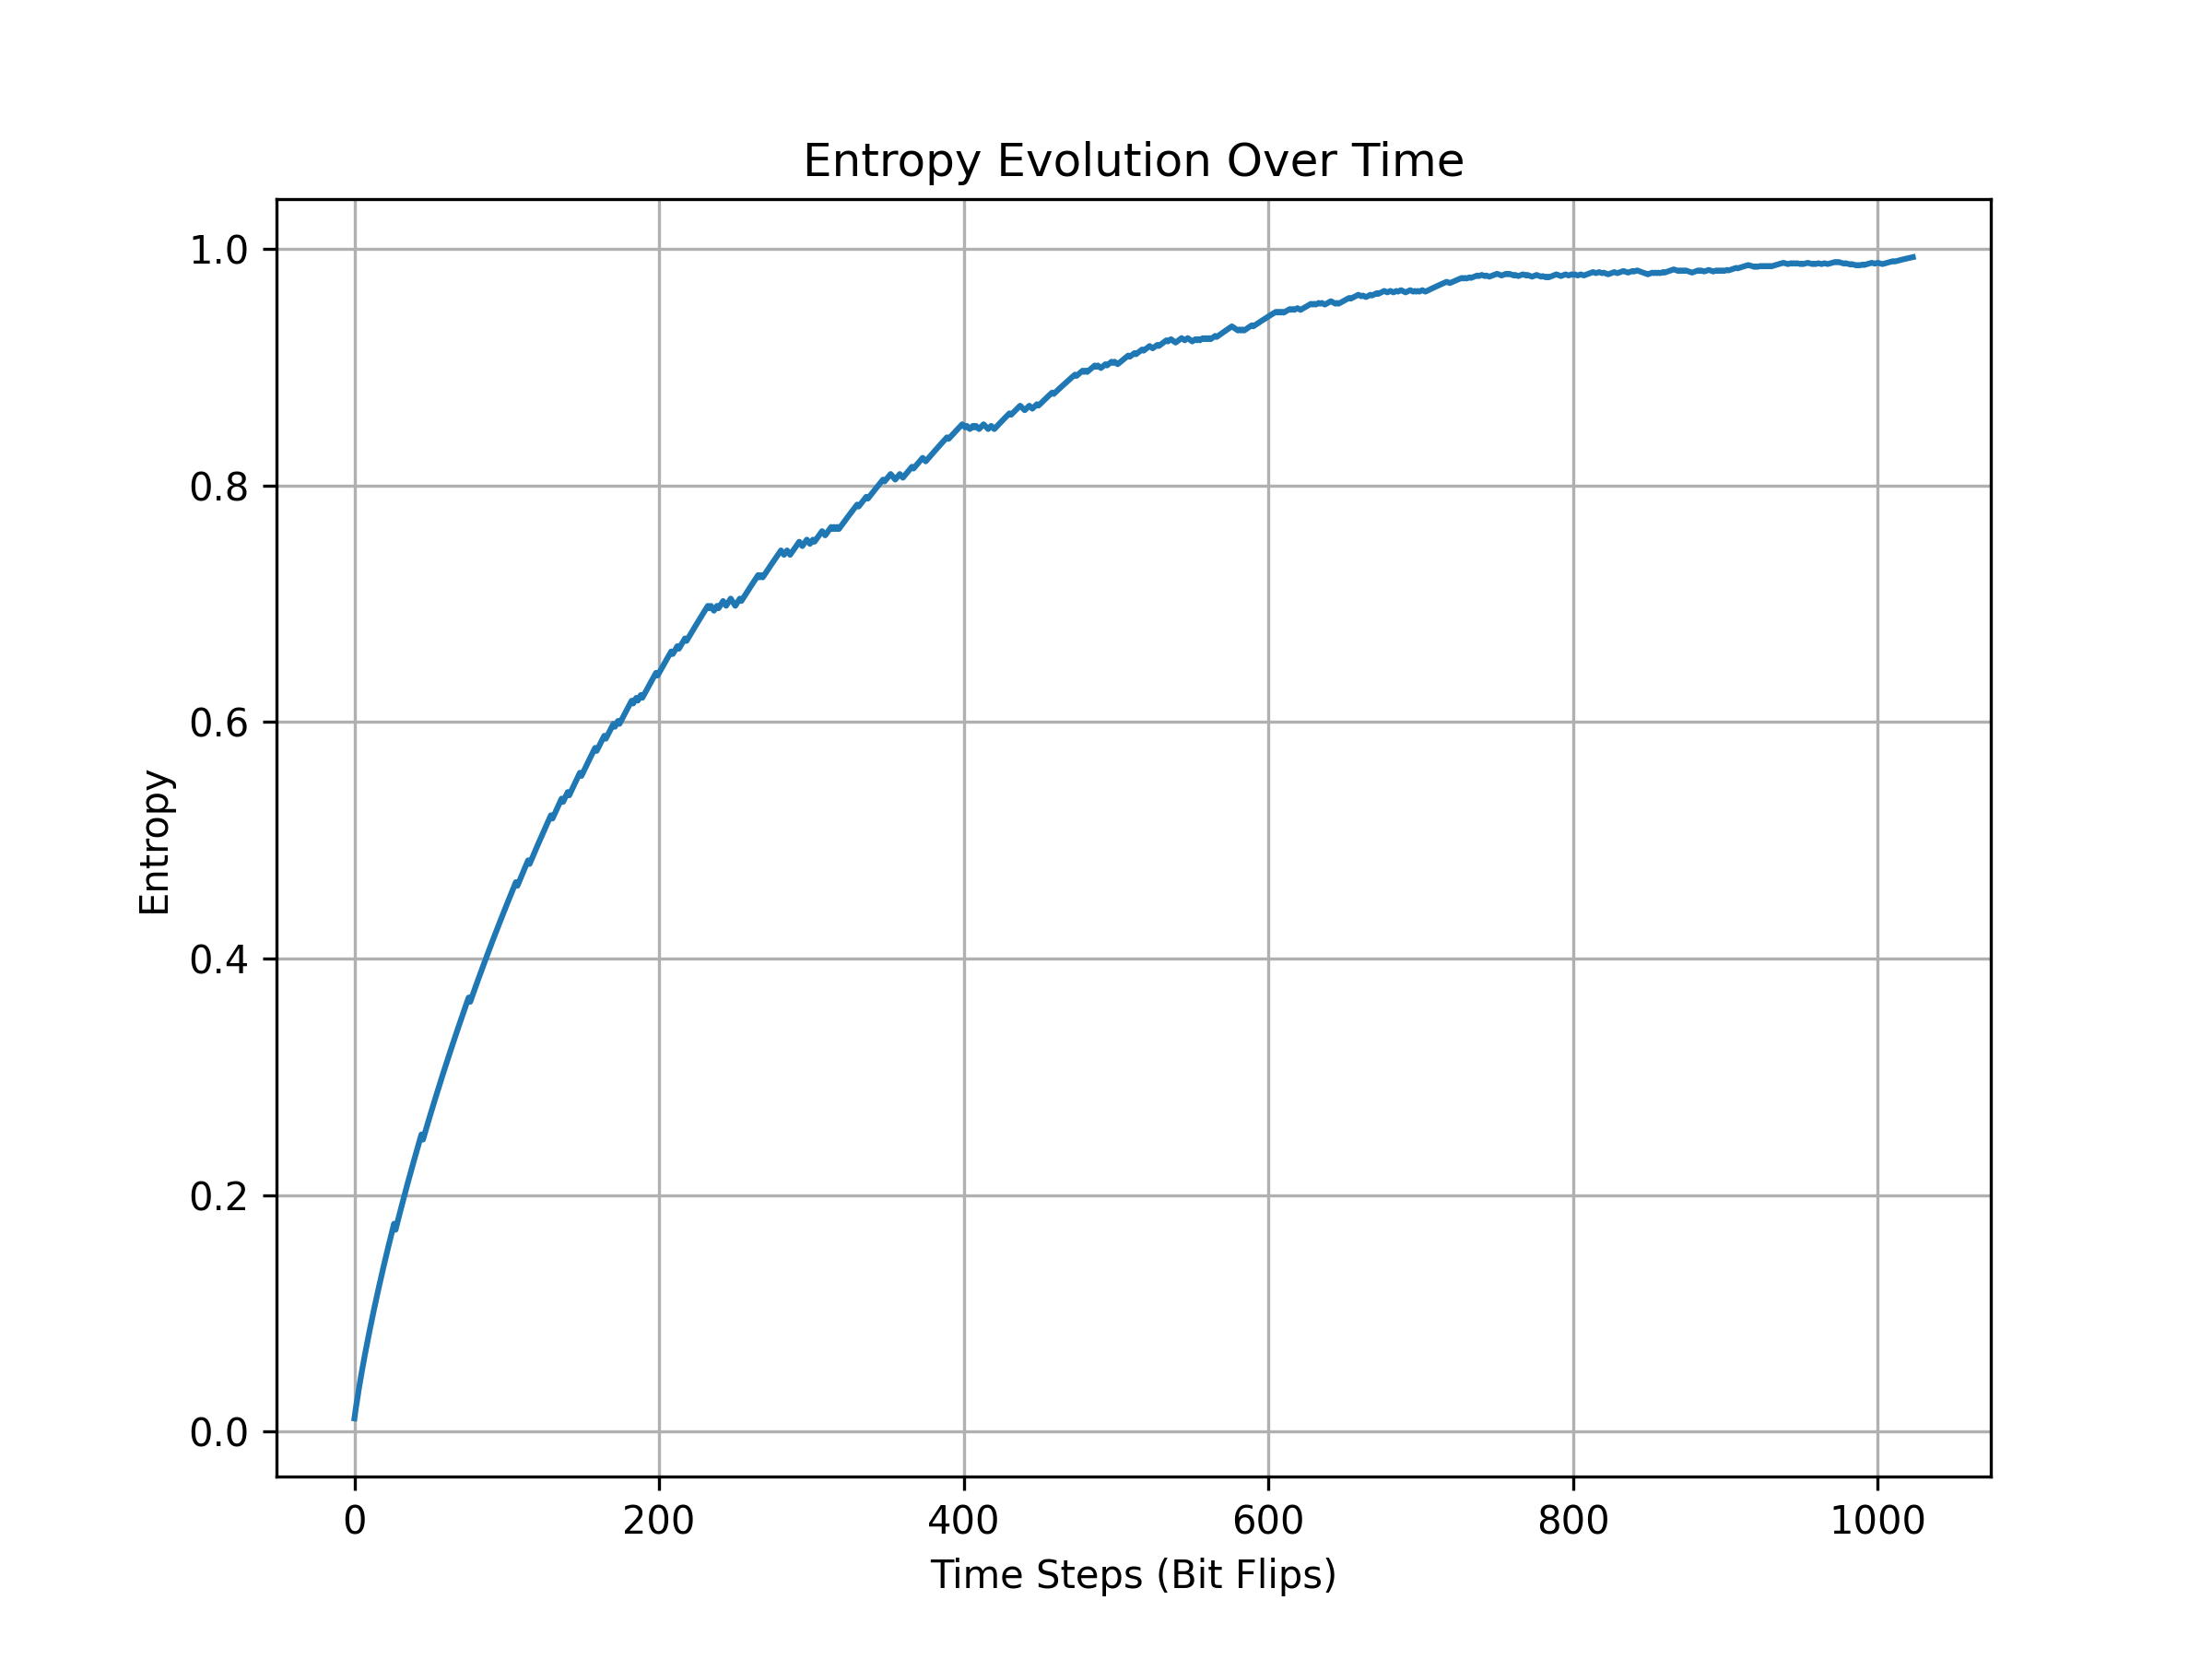
\includegraphics[width=0.8\textwidth]{figures/entropy_evolution_curve.png}
    \caption{Bitstring mutation via bit flips and resulting entropy growth.}
    \label{fig:bitstring-evolution}
\end{figure}

\section{Statistical Properties: Lognormal Emergence}

Plotting the number of valid geometric structures against entropy reveals a lognormal-like distribution:

\begin{itemize}
    \item Rapid growth in structure during early entropy increase.
    \item Peak structure formation at intermediate entropy.
    \item Slow saturation as entropy nears maximum.
\end{itemize}

At low entropy, only simple structures (elementary particles) appear. As entropy rises, more complex entities (atoms, molecules) emerge. These patterns provide insight into how complexity arises naturally from entropy increase.

\begin{figure}[h!]
    \centering
    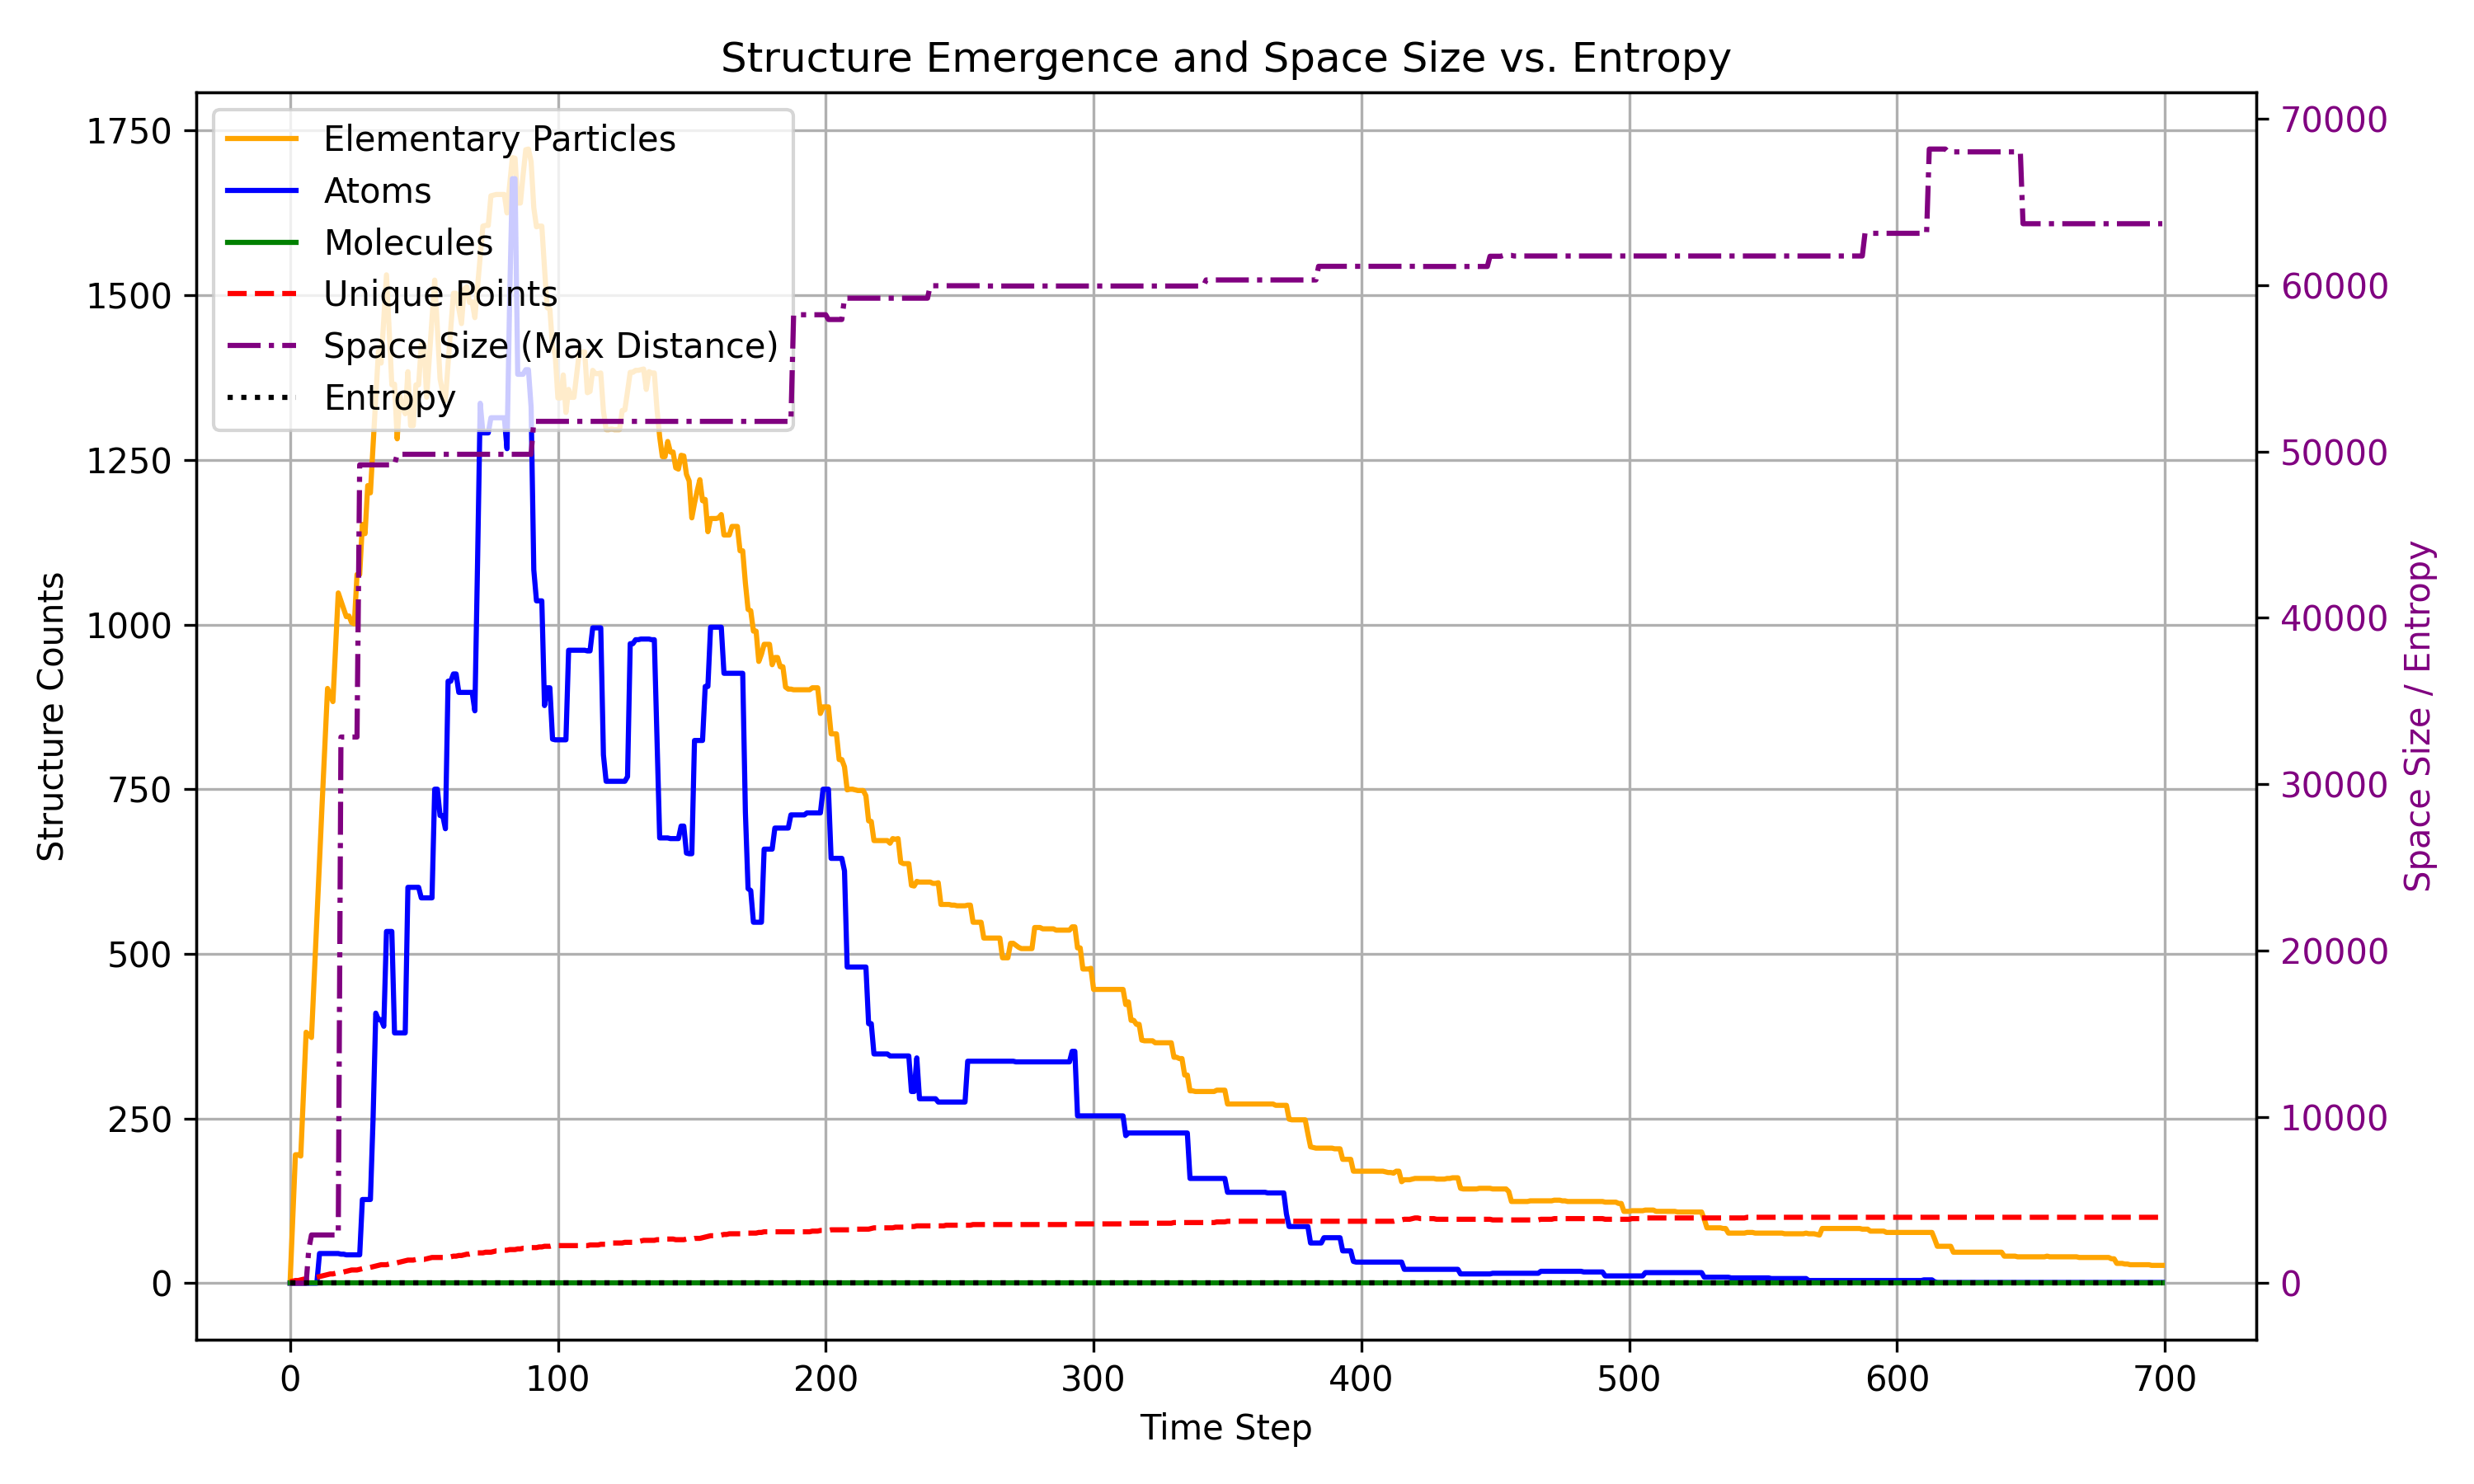
\includegraphics[width=0.8\textwidth]{figures/entropy_to_matter.png}
    \caption{Structure count vs. entropy. The emergence follows a lognormal-like distribution.}
    \label{fig:lognormal-structure}
\end{figure}

The simulation source code is available at \url{http://github.com/juhakm/emergence_of_spacetime.py}.

\section{Implications for Gravity}

Although the model is abstract and lacks direct predictive power, it reveals regularities in the evolution of bitstring-based universes. Notably, the emergence of a lognormal structure distribution near the entropy minimum suggests that the singularity is not a point of breakdown, but one of perfect informational smoothness. In this regime, the entropy landscape offers no persistent structures—no particles, no time evolution, and therefore no gravitational field.

This conclusion contrasts sharply with conventional theories. General Relativity predicts infinite curvature at the singularity, while quantum mechanics denies the possibility of a zero-entropy ground state. Our simulation, however, begins from such a state and demonstrates that structure emerges only as entropy increases.

We interpret this contradiction not as a flaw in the model, but as a possible sign that prevailing physical theories may be incomplete or inapplicable at informationally fundamental scales.

\section*{Conclusion}

Our findings suggest that both General Relativity and Quantum Mechanics break down at the singularity not because of mathematical difficulties, but because their assumptions fail in a regime where the universe is fundamentally informational. Rather than infinities or quantum fluctuations, we observe a smooth entropy profile from which spacetime and matter emerge only after entropy begins to rise.

In this view, spacetime is not the backdrop for information to evolve; rather, information is the substance from which spacetime itself emerges. Particles arise as statistical structures from evolving bitstrings. If the observed lognormal distribution of emergent structures holds, it may become possible to define spacetime metrics using statistical methods rather than relying solely on existing theories of gravity.

It is important to acknowledge that predictions about gravity at the singularity remain, by definition, beyond direct observational verification. Singularities are theoretical boundaries where classical physics breaks down and measurement is impossible. This study was motivated by earlier work in which we demonstrated that a physical (geometric) description and an information-theoretic (computational) trace are two distinct representations of the same underlying structure \cite{meskanen2020}. That result suggested the possibility of extending the information-theoretic description through the singularity—where physical models cannot proceed. The current simulation was developed to explore that informational extension. While abstract, it recovers qualitative features consistent with known physical laws and offers a coherent extrapolation beyond the point at which those laws fail.

\section{Future Work}

Planned extensions include:

\begin{itemize}
    \item \textbf{Toward a Unified Framework:} Investigate how both GR (which fails due to singularities) and QM (which assumes nonzero initial entropy) might be subsumed by a unified information-theoretic model that explains curvature and entanglement as emergent phenomena.

    \item \textbf{Emergence of Consciousness:} A theory of everything must also address human consciousness. We will explore how subjective experience and stable physical laws may arise only in a narrow class of simulations, potentially explaining fine-tuning without invoking external causes.

    \item \textbf{Empirical Consequences:} While currently abstract, we will identify potential empirical consequences—such as specific entropy distributions in microstructure or deviations from physical law near black hole singularities—that could support or falsify the model.
\end{itemize}

Ultimately, we aim to replace geometric and probabilistic formulations of the universe with a single, consistent, observer-relative model rooted in finite information and computability.

\end{document}
